\documentclass[UKenglish
  pdftex                    % Option for graphicx
  dvipsnames                % Option for xcolor
]{beamer}

\usepackage[utf8]{inputenx} % For æ, ø, å
\usepackage{microtype}      % Forbedret typografi
\usepackage{amssymb}        % Matematiske symboler
\usepackage{mathtools}      % Matematiske symboler
\usepackage[absolute, overlay]{textpos} % Vilkårlig plassering
\setlength{\TPHorizModule}{\paperwidth} % Textposenheter
\setlength{\TPVertModule}{\paperheight} % Textposenheter
\usepackage{tikz}
\usetikzlibrary{overlay-beamer-styles}  % Overlayeffekter for TikZ

%\usepackage[pdftex]{graphicx} % Insert PDF image

% This adds colour into LaTeX.
%\usepackage[dvipsnames]{xcolor}
% Define some commonly used colours
\definecolor{forestgreen}{HTML}{228B22}
\definecolor{Rblue}{RGB}{35,105,189}

%//ref https://tex.stackexchange.com/questions/42619/x-mark-to-match-checkmark/42620
\usepackage{pifont} % Insert tick and cross marks
\newcommand{\tmark}{\textcolor{blue}{\ding{51}}}
\newcommand{\xmark}{\textcolor{red}{\ding{55}}}
\newcommand{\vmark}{\textcolor{forestgreen}{\ding{228}}}

% This is for the bibliography/reference list. Use APA 7.
\usepackage[british]{babel}% For oversettelser
\usepackage{csquotes}
\usepackage[style=apa]{biblatex}
\addbibresource{~/uio/pc/Dokumenter/PhD/Bibliography/Master.bib}

\newcommand{\cR}{
\includegraphics[width=1.1em]{Figures/R.png}\ }
\newcommand{\CR}{
\includegraphics[width=1.1em]{Figures/R.png}}
\newcommand{\pk}[1]{\textcolor{Rblue}{\textsf{#1}}}

% Always load cleveref last last
\usepackage[nameinlink,noabbrev,capitalise]{cleveref}

% Fjern logo fra ordinære slides med \usetheme[NoLogo]{MathDept}
\usetheme{MathDept}

\author{Tony C. A. Tan}
\title{Missing Data Treatment}
\subtitle{A hand-on illustration using \cR package \pk{mice}}
\date{28 Feburary 2022}

\begin{document}

\section*{Structure}
%%%%%%%%%%%%%%%%%%%%%%%%%%% Begin TOC %%%%%%%%%%%%%%%%%%%%%%%%%%%
%%                                                             %%
\begin{frame}%[allowframebreaks]
\frametitle{Structure}

  \tableofcontents%[currentsection]

\end{frame}
%%                                                             %%
%%%%%%%%%%%%%%%%%%%%%%%%%%%% End TOC %%%%%%%%%%%%%%%%%%%%%%%%%%%%

\section{Background}

\subsection{Summary}
%%%%%%%%%%%%%%%%%%%%%%%%%% Begin Slide %%%%%%%%%%%%%%%%%%%%%%%%%%
%%                                                             %%
\begin{frame}\frametitle{Summary}

\begin{itemize}

  \item Complete-case analyses:
  \begin{itemize}
    \item[\xmark] Wasteful
    \item[\xmark] Biased
  \end{itemize}

  \item Two approaches:
  \begin{itemize}
    \item[\ding{192}] Joint modelling \parencite[JM,][]{schafer:1997}
    \item[\ding{193}] Fully conditional specification (FCS)
    \item[\ding{43}] FCS aka multivariate imputation by chained equations \parencite[MICE,][]{vanbuuren:2011}
  \end{itemize}

  \item Existing \cR packages:
  \begin{itemize}
    \item[\ding{228}] \pk{Amelia}, \pk{Hmisc}, \pk{jomo}, \pk{mi}, \pk{mice}, \pk{norm}, \pk{norm2}, \pk{pan}
    \item[\ding{45}] See Table 5.1, \textcite{kleinke:2020} (p. 134) for popularity contest across various MI packages
    \item[\ding{45}] See Table 6, \textcite{grund:2018} (pp. 134--135) for missing data treatment for multilevel models
  \end{itemize}

\end{itemize}

\end{frame}
%%                                                             %%
%%%%%%%%%%%%%%%%%%%%%%%%%%% End Slide %%%%%%%%%%%%%%%%%%%%%%%%%%%

\subsection{Data Missing Mechanism}
%%%%%%%%%%%%%%%%%%%%%%%%%% Begin Slide %%%%%%%%%%%%%%%%%%%%%%%%%%
%%                                                             %%
\begin{frame}\frametitle{Data Missing Mechanism \normalsize\parencite{rubin:1976}}

\begin{itemize}
  \item Missing completely at random (\textbf{MCAR})
    \begin{itemize}
      \item[\ding{46}] missingness of variables is independent of the variables considered in the study
      \item[\tmark] no treatment required, complete-case analyses valid and unbiased
    \end{itemize}

    \item Missing at random (\textbf{MAR})
  \begin{itemize}
    \item[\ding{46}] missingness depends exclusively on observable variables
    \item[\tmark] the assumption behind most MI procedures, including \pk{mice}
  \end{itemize}

  \item Missing not at random (\textbf{MNAR})
  \begin{itemize}
    \item[\ding{46}] missingness depends on unobservable but important variables of interest in the study
    \item[\tmark] exact treatment rather complicated \parencite{rose:2013}
    \item[\tmark] in practice: introduce lots of covariates and hope MNAR $\approxeq$ MAR
  \end{itemize}

  \item[\ding{108}] Ignorable = \{ MCAR, MAR \}; Nonignorable = \{ MNAR \}
\end{itemize}

\end{frame}
%%                                                             %%
%%%%%%%%%%%%%%%%%%%%%%%%%%% End Slide %%%%%%%%%%%%%%%%%%%%%%%%%%%

\section{The \pk{mice} Package}

\subsection{\pk{mice} Process}
%%%%%%%%%%%%%%%%%%%%%%%%%% Begin Slide %%%%%%%%%%%%%%%%%%%%%%%%%%
%%                                                             %%
\begin{frame}\frametitle{\pk{mice} Process \normalsize\parencite{vanbuuren:2011}}

\begin{figure}
  \centering
  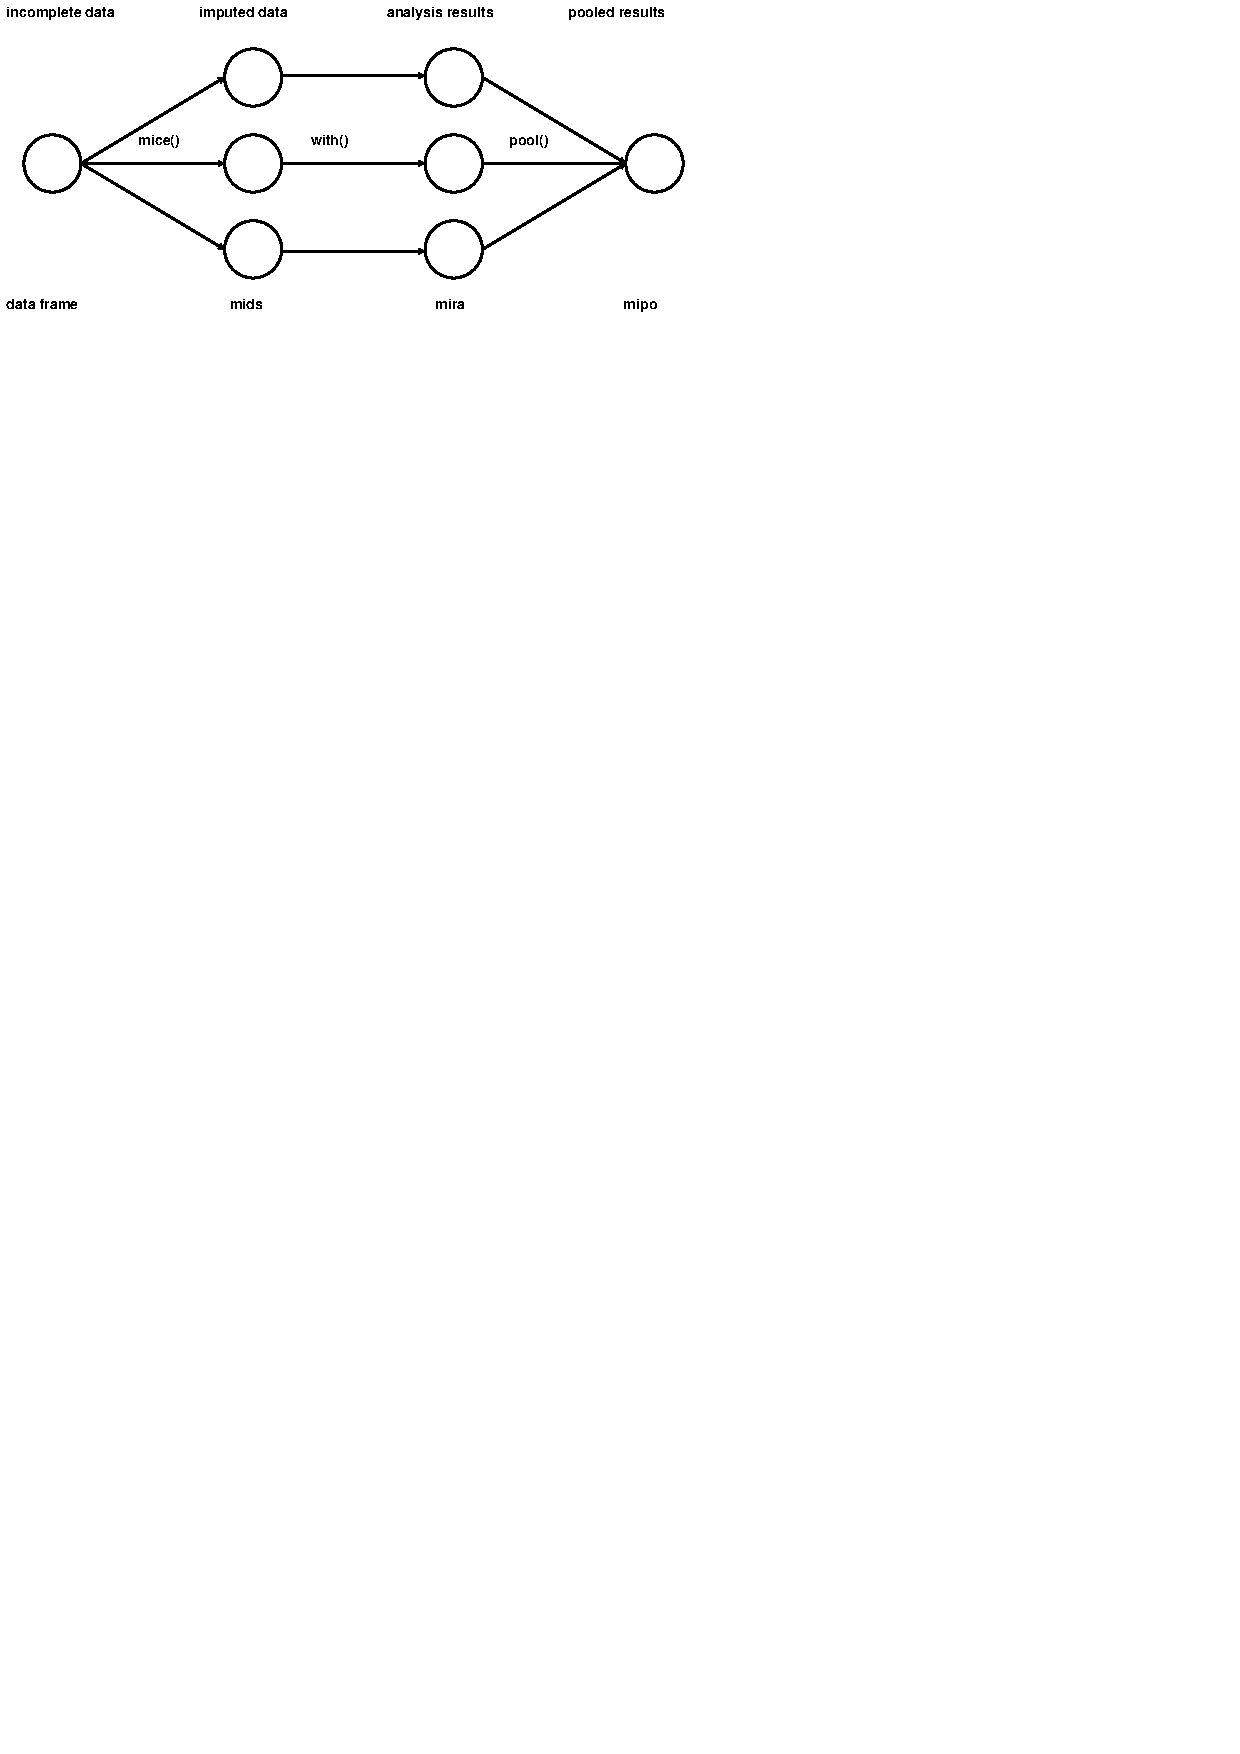
\includegraphics[width=\textwidth]{./Figures/sketch.pdf}
\end{figure}

\end{frame}
%%                                                             %%
%%%%%%%%%%%%%%%%%%%%%%%%%%% End Slide %%%%%%%%%%%%%%%%%%%%%%%%%%%

\section*{Reference}
%%%%%%%%%%%%%%%%%%%%%%%% Begin Reference %%%%%%%%%%%%%%%%%%%%%%%%
%%                                                             %%
\begin{frame}[allowframebreaks]
\frametitle{References}

\printbibliography

\end{frame}
%%                                                             %%
%%%%%%%%%%%%%%%%%%%%%%%%% End Reference %%%%%%%%%%%%%%%%%%%%%%%%%

\end{document}
